\chapter{Laboratory 02: solution}

In this problem we assume that the plant to be identified is exactly described as a discrete-time
LTI models described by the following transfer function (in the \(q^{-1}\) operator):
\[
G_p(q^{-1}) = \frac {\theta_2}{1 + \theta_1q^{-1}}
\]
where
\[
\theta = \left[-0.5 2 \right]
\]
Now, it is required to compute a set-membership estimation of the parameters of the system by means of the following procedure:\\
Assume that the uncertainty affecting the input output data enters the problem according to an equation error structure. Furthermore, to perform the simulation, assume that collected input sequence \(\tilde{u}\) and the unknwon equation error sequences e are as follows :
\[
\tilde{u} = \left[4,\,-3,\,2,\, 1 \right]^T
\]
and
\[
e = \left[0.05,\,-0.25,\,0.3,\,-0.5 \right]^T
\]
Perform a simulation of model in order to collect the input and output data to be used for identification. The output sequence \(tilde{y}\) has to be computed according to the following equation (equation error structure):\\
Based on the transfer function at hand the difference equation of the system is as follow:
\[
y(k) = -\theta_1y(k-1) + \theta_2u(k)
\]
Considering an \textit{Equation-Error} structure for the noise, the following relationship is obtained:
\[
\tilde{y}(k) = -\theta_1 \tilde{y}(k-1) + \theta_2u(k) + e(k)
\]
Where it is assumed that the error \(e\) is known to be bounded as \(|e(k)|\leq \Delta e\) and assuming as initial condition \(\tilde{y}\).

Considering the difference equation of the system, the following information can be obtained:\\
\begin{itemize}
\item \(n_a = 1\) which represent the order of the system, which corresponds to the number of previous samples of \(y\) needed to express the difference equation of the system.
\item \(n_b\) the number of input samples in the difference equation.
\item \(t_{min} = \max(\left[n_a +1, n_b\right]\)
\end{itemize}
MATLAB code for simulation of the system is as follows:

\begin{example}
\begin{lstlisting}[caption=Set-membership estimation with theta bounds and simulation]
close all
clear variables
clc
format compact

%% Defining system
z = tf('z',1);
theta = [-0.5 2];
Gp = theta(2)/(1 + theta(1)*z)

u_tilde = [4 -3 2 1]';
e = [0.05 -0.25 0.3 -0.5]';

%% Simulation
% y_tilde(k) = -theta_1*y_tilde(k-1) + theta_2 u_tilde(k) + e(k)
na = 1; % The number of state variables or last samples of y
nb = 1; % The number of past inputs
N = 4;
t_min = max([na+1 , nb]);
y_tilde = zeros(4,1); 
% Initial value

for k = t_min:N
    y_tilde(k) = -theta(1)*y_tilde(k-1) + theta(2)*u_tilde(k) + e(k);
end

%% Upper and lower bound
delta_e = 0.5;
y_up = y_tilde + delta_e;
y_low = y_tilde - delta_e;
plot(1:N, [y_up, y_tilde, y_low])
\end{lstlisting}
\end{example}

In order to obtain \textit{Feasible Uncertainty Set}, it is required to do the following manipulations, considering the definition of FPS we have:
\[
\mathbb{D}_\theta = \left\{ \theta | \tilde{y}(k) + \theta_1 \tilde{y}(k-1) + \theta_2\tilde{u}(k)| \leq \Delta e \forall k \right\}  
\]
Writing exampding the equations for \(t_{min}\) to \(N = 4\), which is the number of samples, we obtain:
\begin{align*}
|\tilde{y}(2) + \theta_1 \tilde{y}(1) + \theta_2\tilde{u}(2)| &\leq \Delta e \\
|\tilde{y}(3) + \theta_1 \tilde{y}(2) + \theta_2\tilde{u}(3)| &\leq \Delta e \\
|\tilde{y}(4) + \theta_1 \tilde{y}(3) + \theta_2\tilde{u}(4)| &\leq \Delta e
\end{align*}
and therefore,
\begin{align*}
-\Delta e - \tilde{y}(2) \geq \theta_1 \tilde{y}(1) + \theta_2\tilde{u}(2) &\leq \Delta e - \tilde{y}(2) \\
-\Delta e - \tilde{y}(3) \geq \theta_1 \tilde{y}(2) + \theta_2\tilde{u}(3) &\leq \Delta e - \tilde{y}(3) \\-\Delta e - \tilde{y}(4) \geq \theta_1 \tilde{y}(3) + \theta_2\tilde{u}(4) &\leq \Delta e - \tilde{y}(4) 
\end{align*}

In each of these relationships, each inequality is a constraint in parameter space that needs to be satisfied so that the equation error becomes less that \(\Delta e\). For finding \(\mathbb{D}_\theta\) in the parameter space, we can consider inequalities as equality, and by doing so, we obtain the equation of 3 pairs of parallel lines on the parameter space, which in this case is a two-dimensional plane. After writing the following MATLAB code, the intersections of all the regiones between the top bound and lower bounds lead to FPS. The plot of the feasible uncertaintly set in the parameter space is as follows:
\begin{example}
\begin{lstlisting}
%% Theta_1 variation
theta_1 = linspace(-5, 5, 1000);
figure,
hold on
for k = t_min:N
    theta_2_up = (+delta_e + y_tilde(k) + theta_1*y_tilde(k-1)) / u_tilde(k);
    theta_2_low = (-delta_e + y_tilde(k) + theta_1*y_tilde(k-1)) / u_tilde(k);
    plot(theta_1, theta_2_low, 'b')
    plot(theta_1, theta_2_up, 'r')
end

%% Brute-force approach (not recommended)
figure,
hold on
for theta_1 = -100:0.01:100
    for theta_2 = -100:0.01:100
        for k = t_min:N
            f = 1; % Flag
            if(abs(y_tilde(k) + theta_1*y_tilde(k-1) - theta_2*u_tilde(k)) > delta_e)
                f = 0;
                break
            end
        end
        if (f == 1)
            plot(theta_1, theta_2, '+');
        end
    end
end
\end{lstlisting}
\end{example}


\begin{figure}[htbp]  % "h" for here, "t" for top, "b" for bottom, "p" for float page
    \centering
    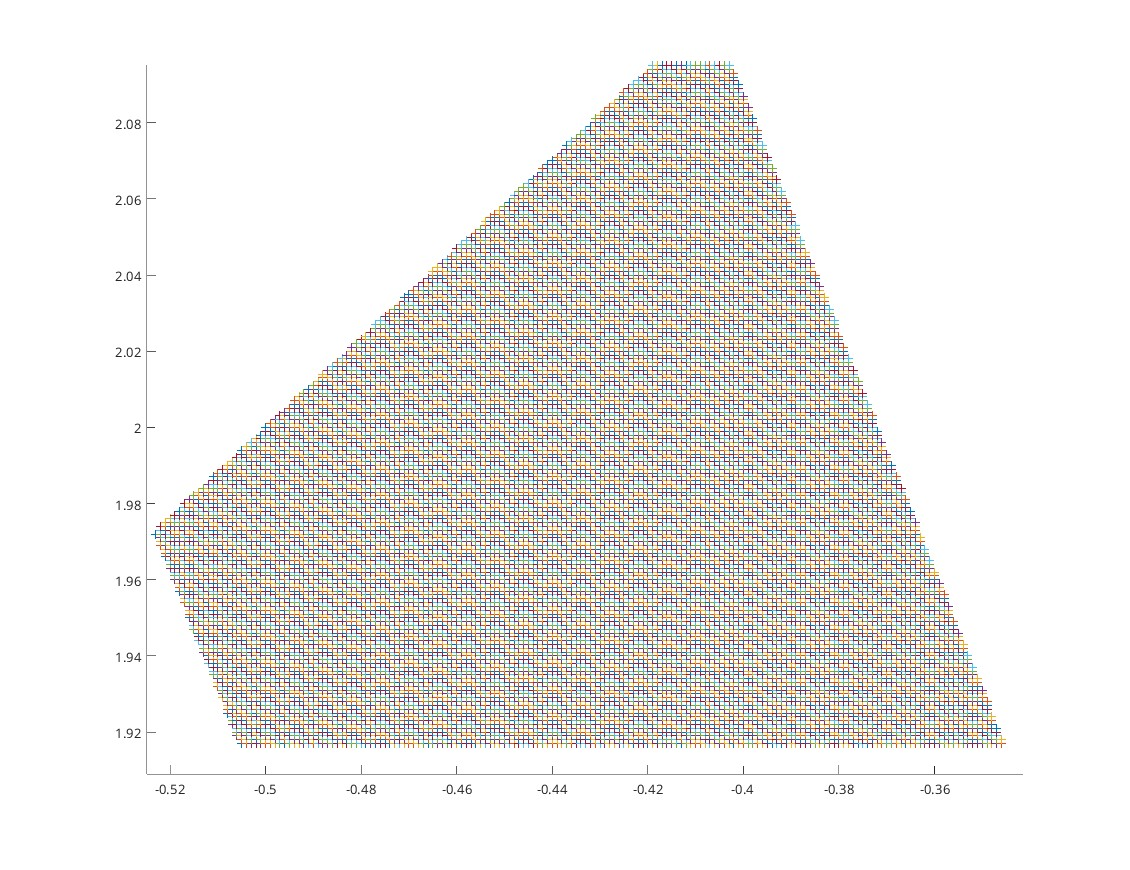
\includegraphics[width=0.65\textwidth]{images/FPS.jpg}
    \caption{FPS represented in the parameter space; the horizontal axis is \(\theta_1\) and the vertical axis is \(\theta_2 \)}
    \label{fig:PFS}
\end{figure}

It can be seen that the "real value" of the parameters is one of point at the top left corner of the \(\mathbb{D}_\theta\).

